\documentclass[a4paper,12pt]{scrbook} % preambuła
\usepackage[polish]{babel}
\usepackage[utf8]{inputenc} % utf8, cp1250
\usepackage{pslatex}
\usepackage[T1]{fontenc}
\usepackage{times}
\usepackage{geometry}
\usepackage{algorithm}
\usepackage{graphicx}
\usepackage{xcolor}
\usepackage{wrapfig}
\usepackage{amsmath}
\usepackage{subcaption}
\usepackage{algpseudocode}
\usepackage{pgfplots}
\newgeometry{tmargin=1.5cm, bmargin=1.5cm, lmargin=1.5cm, rmargin=1.5cm}

\begin{document}
\section{Indukcyjność}.\\
Indukcyjność określa zdolność obwodu do wytwarzania strumienia pola magnetycznego $\phi$ powstającego w wyniku przepływu przez obwód prądu elektrycznego $I$. Jednostką indukcyjności jest henr ($H = \frac{kg \cdot m^2}{A^2 \cdot s^2}$). 

\begin{center}
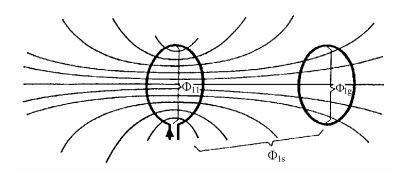
\includegraphics[scale=0.7]{rys1.jpg}
\end{center}

Na rysunku powyżej przedstawiono dwie cewki umieszczone blisko, które mogą oddziaływać na siebie wzajemnie. Pole magnetyczne wytworzone w jednej cewce przenika całkowicie lub częściowo przez drugą cewkę. Załóżmy, że prąd o natężeniu $i_1$ w cewce pierwszej (o $N_1$ zwojach) wytwarza w niej strumień indukcji pola magnetycznego $\phi_{11}$. Część tego strumienia $\phi_{1g}$ przecina drugą cewkę (o $N_2$ zwojach), pozostała część strumienia $\phi_{1s}$ - zwana strumieniem rozproszenia zamyka się dokoła cewki (1) w taki sposób, że linie indukcji nie obejmują cewki (2). Całkowity strumień wytwarzany przez cewkę (1) jest więc sumą dwóch składowych $ \phi_{11} = \phi_{1g} + \phi_{1s}$ (wzor 1).

\paragraph{Indukcyjność własna oraz wzajemna}.\\
Stosunek strumienia magnetycznego skojarzonego z danym uzwojeniem do prądu, który wywołuje ten strumień, nazywamy indukcyjnością własną uzwojenia $L_1 = \frac{N_1 \cdot \phi_{11}}{i_1}$ (wzor 2).

Strumień magnetyczny $\phi_{1g}$ (czyli strumień przez cewkę drugą, ale związany z prądem w cewce pierwszej) sprzęga się z $N_2$ zwojami cewki drugiej.

\noindent
Indukcyjność wzajemną cewki pierwszej z cewką drugą można wyrazić zależnością $M_{12} = \frac{N_2 \phi_{1g}}{i_1}$ (wzor 3). Analogicznie dla drugiej cewki $L_2 = \frac{N_2 \cdot \phi_{22}}{i_2}$ oraz $M_{21} = \frac{N_1 \phi_{2g}}{i_2}$ (wzory 4).

Z podstawowych praw elektromagnetyzmu wynika, że indukcyjności wzajemne $M_{12}, M_{21}$ są zawsze takie same $M = M_{12} = M{21}$. Gdzie wielkość M nazywamy indukcyjnością wzajemną dwóch cewek.

Rozkład całkowitego strumienia magnetycznego na strumień główny i strumień rozproszenia jest punktem wyjścia do określenia indukcyjności głównej $L_{1g}$ i indukcyjności rozproszenia $L_{1s}$ jest punktem wyjścia do określenia indukcyjności głównej $L_{1g}$ i indukcyjności rozproszenia $L_{1s}$\\
\begin{equation}
\begin{gathered}
L_{1g} = \frac{N_1 \phi_{1g}}{i_1}\\
L_{1s} = \frac{N_1 \phi_{1s}}{i_1}\\
\text{Wykorzystując wzory (1) - (4) można wykazać, że: } \\
L_1 = L_{1g} + L_{1s} \\
L_2 = L_{2g} + L_{2s} \\
M = \sqrt{L_{1g}L_{2g}}
\end{gathered}
\end{equation}
Więc indukcyjność wzajemna jest średnią geometryczną obu indukcyjności głównych. Oznaczmy współczynnik sprzężenia obu cewek jako $k$ wtedy $M = k \sqrt{L_1 L_2}$.

Indukcyjność wzajemna cewek powietrznych (bez rdzenia magnetycznego) zależy od:
\begin{enumerate}
\item{kształtu geometrycznego cewek}
\item{wzajemnego usytuowania cewek}
\item{liczby zwojów}
\end{enumerate}

Gdy przestrzeń otaczającą cewki wypełnimy, przynajmniej częściowo, substancją magnetyczną o przenikalności względnej $\mu_r >> 1$ wtedy strumienie pola magnetycznego i w konsekwencji wartości indukcyjności ulegają zwiększeniu.
\end{document}